% Standalone TikZ source for the end-to-end architecture figure.
% Avoids standalone.cls (not installed). Uses article + geometry + shipout
% to produce a tightly cropped PDF.
%
% Compile with:
%   pdflatex fig_architecture.tex   (or ./build.sh fig_architecture.tex)
% to produce fig_architecture.pdf, included via:
%   
\includegraphics[width=0.88\textwidth]{figures/fig_architecture.pdf}

\documentclass{article}
\usepackage[paperwidth=205mm,paperheight=125mm,margin=3mm]{geometry}
\usepackage{tikz}
\usetikzlibrary{arrows.meta, positioning, fit, backgrounds, calc}
\usepackage{amsmath}
\usepackage{amssymb}   % \mathbb

\pagestyle{empty}
\setlength{\parindent}{0pt}
\setlength{\topskip}{0pt}
\setlength{\parskip}{0pt}

\begin{document}
\noindent
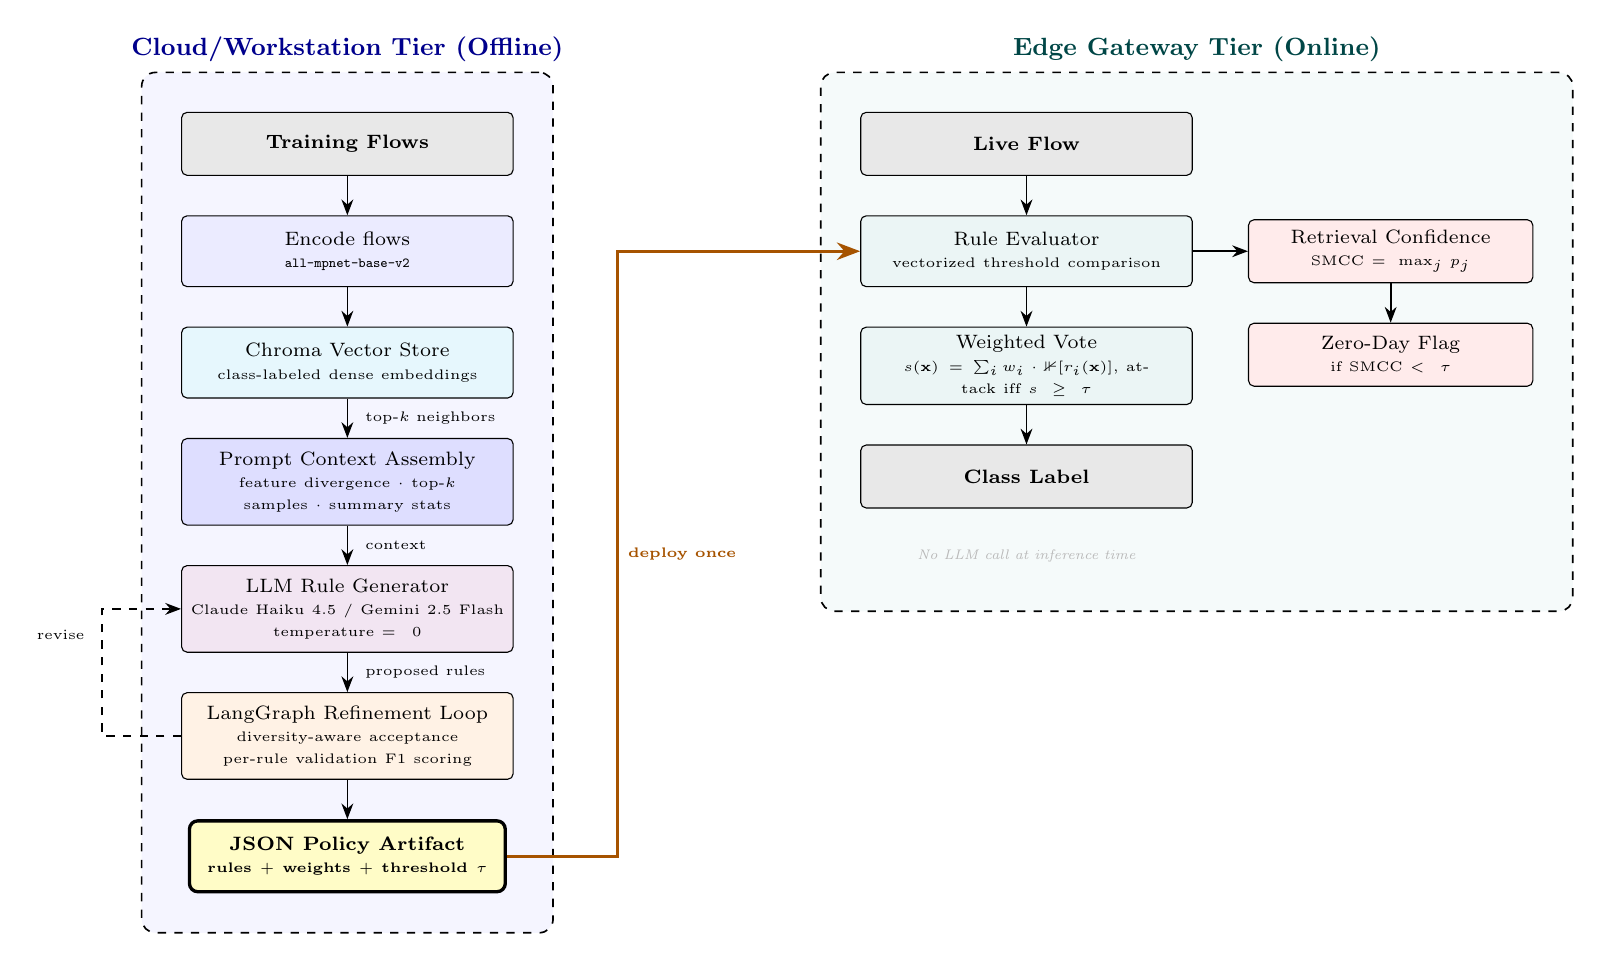
\begin{tikzpicture}[
  >=Stealth,
  node distance = 5mm,
  ionode/.style   = {draw, rounded corners=2pt, fill=gray!18,
                     text width=40mm, align=center,
                     font=\scriptsize\bfseries,
                     inner sep=3pt, minimum height=8mm},
  procnode/.style = {draw, rounded corners=2pt, fill=blue!8,
                     text width=40mm, align=center,
                     font=\scriptsize, inner sep=3pt,
                     minimum height=9mm},
  storenode/.style= {draw, rounded corners=2pt, fill=cyan!10,
                     text width=40mm, align=center,
                     font=\scriptsize, inner sep=3pt,
                     minimum height=9mm},
  ctxnode/.style  = {draw, rounded corners=2pt, fill=blue!13,
                     text width=40mm, align=center,
                     font=\scriptsize, inner sep=3pt,
                     minimum height=11mm},
  llmnode/.style  = {draw, rounded corners=2pt, fill=violet!10,
                     text width=40mm, align=center,
                     font=\scriptsize, inner sep=3pt,
                     minimum height=11mm},
  refnode/.style  = {draw, rounded corners=2pt, fill=orange!10,
                     text width=40mm, align=center,
                     font=\scriptsize, inner sep=3pt,
                     minimum height=11mm},
  artnode/.style  = {draw, very thick, rounded corners=3pt,
                     fill=yellow!22, text width=38mm, align=center,
                     font=\scriptsize\bfseries,
                     inner sep=3pt, minimum height=9mm},
  edgenode/.style = {draw, rounded corners=2pt, fill=teal!8,
                     text width=40mm, align=center,
                     font=\scriptsize, inner sep=3pt,
                     minimum height=9mm},
  flagnode/.style = {draw, rounded corners=2pt, fill=red!8,
                     text width=34mm, align=center,
                     font=\scriptsize, inner sep=3pt,
                     minimum height=8mm},
  arr/.style    = {->, semithick},
  bigarr/.style = {->, very thick},
  grpbg/.style  = {draw, dashed, semithick, rounded corners=5pt,
                   inner sep=5mm},
]

% =============================================
% OFFLINE COLUMN (left)
% =============================================
\node[ionode]    (traindata) {Training Flows};
\node[procnode,  below=of traindata] (encode)  {Encode flows\\{\tiny\texttt{all-mpnet-base-v2}}};
\node[storenode, below=of encode]    (chroma)  {Chroma Vector Store\\{\tiny class-labeled dense embeddings}};
\node[ctxnode,   below=of chroma]    (ctx)     {Prompt Context Assembly\\{\tiny feature divergence~$\cdot$~top-$k$ samples~$\cdot$~summary stats}};
\node[llmnode,   below=of ctx]       (llm)     {LLM Rule Generator\\{\tiny Claude Haiku 4.5 / Gemini 2.5 Flash}\\{\tiny temperature $= 0$}};
\node[refnode,   below=of llm]       (refine)  {LangGraph Refinement Loop\\{\tiny diversity-aware acceptance}\\{\tiny per-rule validation F1 scoring}};
\node[artnode,   below=of refine]    (json)    {JSON Policy Artifact\\{\tiny rules~$+$~weights~$+$~threshold~$\tau$}};

% =============================================
% ONLINE COLUMN (right)
% =============================================
\node[ionode,    right=44mm of traindata] (liveflow) {Live Flow};
\node[edgenode,  below=of liveflow]       (ruleeval) {Rule Evaluator\\{\tiny vectorized threshold comparison}};
\node[edgenode,  below=of ruleeval]       (wvote)    {Weighted Vote\\{\tiny $s(\mathbf{x})=\sum_i w_i\cdot\mathbb{1}[r_i(\mathbf{x})]$,~attack iff~$s\!\geq\!\tau$}};
\node[ionode,    below=of wvote]          (clabel)   {Class Label};
% SMCC / zero-day branch
\node[flagnode,  right=7mm of ruleeval]   (smcc)     {Retrieval Confidence\\{\tiny SMCC $=\max_j\,p_j$}};
\node[flagnode,  below=5mm of smcc]       (zdflag)   {Zero-Day Flag\\{\tiny if SMCC $< \tau$}};
% annotation
\node[font=\tiny\itshape, text=gray!55, align=center,
      below=4mm of clabel] (nollm) {No LLM call at inference time};

% =============================================
% OFFLINE ARROWS
% =============================================
\draw[arr] (traindata) -- (encode);
\draw[arr] (encode)    -- (chroma);
\draw[arr] (chroma)    -- (ctx)
    node[midway, right, font=\tiny, xshift=1mm]{top-$k$ neighbors};
\draw[arr] (ctx)       -- (llm)
    node[midway, right, font=\tiny, xshift=1mm]{context};
\draw[arr] (llm)       -- (refine)
    node[midway, right, font=\tiny, xshift=1mm]{proposed rules};
\draw[arr] (refine)    -- (json);
% Refinement loop: left, up, right back to LLM
\draw[arr, dashed]
    (refine.west) -- ++(-10mm, 0) |- (llm.west)
    node[pos=0.4, left, font=\tiny, xshift=-1mm]{revise};

% =============================================
% JSON BRIDGE ARROW
% =============================================
\draw[bigarr, orange!65!black]
    (json.east) -- ++(14mm, 0) |- (ruleeval.west)
    node[pos=0.25, right, font=\tiny\bfseries,
         text=orange!65!black]{deploy once};

% =============================================
% ONLINE ARROWS
% =============================================
\draw[arr] (liveflow)      -- (ruleeval);
\draw[arr] (ruleeval)      -- (wvote);
\draw[arr] (wvote)         -- (clabel);
\draw[arr] (ruleeval.east) -- (smcc.west);
\draw[arr] (smcc)          -- (zdflag);

% =============================================
% GROUP BACKGROUND BOXES
% =============================================
\begin{scope}[on background layer]
  \node[grpbg, fill=blue!4,
        fit=(traindata)(encode)(chroma)(ctx)(llm)(refine)(json),
        label={[font=\small\bfseries, text=blue!55!black]above:%
               Cloud/Workstation Tier (Offline)}] (offbox) {};
  \node[grpbg, fill=teal!4,
        fit=(liveflow)(ruleeval)(wvote)(clabel)(smcc)(zdflag)(nollm),
        label={[font=\small\bfseries, text=teal!55!black]above:%
               Edge Gateway Tier (Online)}] (onbox) {};
\end{scope}

\end{tikzpicture}
\end{document}
